\documentclass[10pt,letterpaper]{article}
\usepackage[margin=0.6in]{geometry}
\usepackage{graphicx}
\usepackage{booktabs}
\usepackage{enumitem}
\usepackage{hyperref}
\usepackage{xcolor}
\usepackage{amsmath}
\usepackage{tikz}
\usepackage{pgfplots}
\pgfplotsset{compat=1.17}
\usetikzlibrary{shapes,arrows,positioning,fit,backgrounds,patterns}
\usepackage{titlesec}
\usepackage{float}
\usepackage{subcaption}
\titlespacing*{\section}{0pt}{6pt}{2pt}
\titlespacing*{\subsection}{0pt}{4pt}{2pt}
\titlespacing*{\subsubsection}{0pt}{3pt}{1pt}
\setlength{\parskip}{1pt}
\setlength{\floatsep}{4pt}
\setlength{\textfloatsep}{4pt}
\setlength{\intextsep}{4pt}

\hypersetup{
    colorlinks=true,
    linkcolor=blue,
    filecolor=magenta,
    urlcolor=blue,
    citecolor=blue
}

% Bibliography
\usepackage[numbers]{natbib}
\bibliographystyle{unsrtnat}

\title{\textbf{Adaptive RDMA Optimization for Distributed LLM Workloads}\\[0.5em]
\large Adaptive Transport Middleware for Distributed LLM Inference}
\author{Nathan Gopee\\
MS Computer Science, SUNY New Paltz\\
\texttt{gopeen1@newpaltz.edu}\\[1em]
\small Advisors: Dr. Wafi Danesh \& Dr. Ashley Suchy}
\date{February 2026}

\begin{document}

\maketitle

\section{Introduction and Motivation}

Distributed large language model (LLM) inference across multiple GPU nodes requires high-throughput, low-latency inter-node communication. The dominant communication library in this space, NVIDIA NCCL, supports multiple transport backends---including TCP sockets and RDMA via InfiniBand verbs---but selecting and configuring the optimal transport for a given cluster remains a manual and error-prone process. Furthermore, emerging transport technologies such as Tesla's Time-Triggered Protocol over Ethernet (TTPoe) \cite{ttpoe-repo} offer promising latency characteristics but lack turnkey integration with existing inference frameworks.

This work addresses these challenges by building a middleware layer---ScuffedRDMA---that abstracts transport selection for distributed vLLM inference, enabling dynamic switching between TCP, Soft-RoCE, and Tesla TTPoe through a unified interface. Prior profiling of the cluster showed TCP inter-node latency of approximately 1\,ms and Soft-RoCE latency of approximately 190\,$\mu$s, motivating the need for a structured comparison framework. In addition, we integrated RDMA support into the exo peer-to-peer inference framework \cite{exo-github}, providing an alternative deployment path for heterogeneous GPU clusters.

Key contributions include:

\begin{itemize}[noitemsep]
    \item A transport abstraction layer with pluggable backends for TCP, Soft-RoCE, and TTPoe
    \item An NCCL configuration manager for automatic environment setup per transport
    \item A unified benchmark suite for systematic transport comparison
    \item Cluster management scripts that accept a \texttt{--transport} flag for seamless switching
    \item RDMA transport modules for the exo distributed inference framework
\end{itemize}

\section{Middleware Architecture}

\subsection{Design Overview}

The ScuffedRDMA transport middleware provides a clean abstraction over different networking technologies, allowing the same vLLM deployment to switch transports via environment variables or command-line flags. Applications interact with a single unified API at the top level, while the middleware dispatches to the appropriate transport-specific backend underneath.

\begin{figure}[H]
\centering
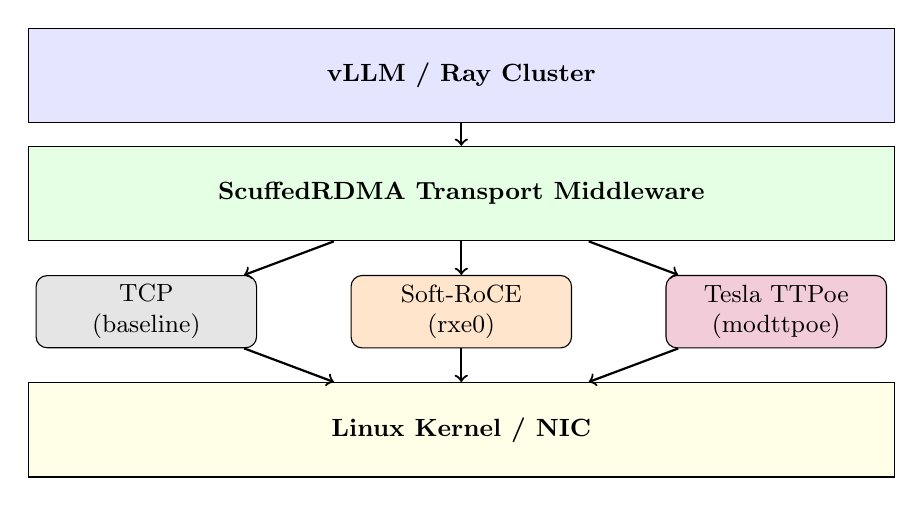
\begin{tikzpicture}[
    node distance=0.8cm,
    box/.style={rectangle, draw, rounded corners, minimum width=2.8cm, minimum height=0.8cm, align=center, font=\small},
    layer/.style={rectangle, draw, minimum width=11cm, minimum height=1.2cm, align=center, font=\small},
    arrow/.style={->, thick}
]
    % Top layer
    \node[layer, fill=blue!10] (vllm) at (0,3) {\textbf{vLLM / Ray Cluster}};

    % Middleware layer
    \node[layer, fill=green!10] (middleware) at (0,1.5) {\textbf{ScuffedRDMA Transport Middleware}};

    % Transport boxes
    \node[box, fill=gray!20] (tcp) at (-4,0) {TCP\\(baseline)};
    \node[box, fill=orange!20] (roce) at (0,0) {Soft-RoCE\\(rxe0)};
    \node[box, fill=purple!20] (ttpoe) at (4,0) {Tesla TTPoe\\(modttpoe)};

    % Bottom layer
    \node[layer, fill=yellow!10] (kernel) at (0,-1.5) {\textbf{Linux Kernel / NIC}};

    % Arrows
    \draw[arrow] (vllm) -- (middleware);
    \draw[arrow] (middleware) -- (tcp);
    \draw[arrow] (middleware) -- (roce);
    \draw[arrow] (middleware) -- (ttpoe);
    \draw[arrow] (tcp) -- (kernel);
    \draw[arrow] (roce) -- (kernel);
    \draw[arrow] (ttpoe) -- (kernel);

\end{tikzpicture}
\caption{ScuffedRDMA transport middleware architecture---applications use a unified API while the middleware handles transport-specific details}
\end{figure}

\subsection{Component Overview}

\begin{table}[H]
\centering
\small
\begin{tabular}{@{}llp{7cm}@{}}
\toprule
\textbf{Component} & \textbf{File} & \textbf{Purpose} \\
\midrule
Transport Base & \texttt{transport\_base.py} & Abstract base class with \texttt{send()}, \texttt{recv()}, \texttt{get\_metrics()} \\
TCP Transport & \texttt{tcp\_transport.py} & Standard socket wrapper with latency measurement \\
RoCE Transport & \texttt{roce\_transport.py} & RDMA verbs wrapper using rdma-core/pyverbs \\
TTPoe Transport & \texttt{ttpoe\_transport.py} & Kernel module loader and character device interface \\
Selector & \texttt{selector.py} & Runtime transport selection and factory \\
NCCL Config & \texttt{nccl\_config.py} & NCCL environment variable management \\
\bottomrule
\end{tabular}
\caption{Middleware component overview}
\end{table}

\section{Transport Abstraction Layer}

\subsection{Base Interface}

The \texttt{TransportBase} class defines the contract that all transport implementations must follow. It is an abstract base class exposing four core operations: \texttt{connect(host, port)} to establish a connection to a remote host, \texttt{send(data)} to transmit a byte buffer and return the number of bytes sent, \texttt{recv(size, timeout)} to receive up to a given number of bytes with an optional timeout, and \texttt{is\_available()} to check whether the transport backend is present on the current system. A companion \texttt{TransportMetrics} data class tracks minimum, maximum, and average latency, total bytes sent and received, and CPU usage, enabling consistent performance reporting across all backends.

\subsection{TCP Transport}

The TCP transport provides the baseline implementation using standard Berkeley sockets. It creates a TCP connection with the \texttt{TCP\_NODELAY} option enabled (disabling Nagle's algorithm) to minimize latency for small transfers typical of tensor metadata exchange. Each \texttt{send()} call measures wall-clock latency using a high-resolution timer and updates the transport metrics accordingly. The \texttt{is\_available()} method always returns true, since TCP sockets are universally available on all Linux systems.

\subsection{Soft-RoCE Transport}

The RoCE transport wraps RDMA verbs operations using pyverbs from rdma-core \cite{rdma-core}. On connection, it opens an RDMA device context for the \texttt{rxe0} software RDMA device, allocates a protection domain and queue pair (QP), and performs out-of-band QP information exchange with the remote peer over a temporary TCP channel. After exchanging QP numbers, LID, and GID information, the queue pair is transitioned through the Init, Ready-to-Receive, and Ready-to-Send states. The \texttt{is\_available()} check verifies that the \texttt{rdma\_rxe} kernel module is loaded on the system.

\subsection{TTPoe Transport}

The TTPoe transport manages the Tesla TTPoe kernel module \cite{ttpoe-repo} and provides a character device interface for data transfer. It loads the \texttt{modttpoe.ko} kernel module via \texttt{insmod}, specifying the network device (e.g., \texttt{eth0}), destination MAC address, and verbosity level as module parameters. Once loaded, the transport opens the \texttt{/dev/ttpoe} character device for read-write access. Data transfer is performed through standard POSIX \texttt{read()} and \texttt{write()} system calls on the file descriptor. The \texttt{is\_available()} method checks whether the compiled kernel module file exists in the expected directory.

\section{NCCL Configuration}

The middleware automatically configures NCCL environment variables based on the selected transport. The \texttt{NCCLConfig} class provides factory methods for each transport type: \texttt{for\_tcp()} disables InfiniBand and sets GDR level to zero; \texttt{for\_softroce(device)} specifies the RoCE device name (defaulting to \texttt{rxe0}) and sets the GID index; \texttt{for\_hardware\_roce(hca)} configures a Mellanox HCA with GPUDirect at GDR level 5. The \texttt{to\_env()} method exports these settings as a dictionary of environment variables suitable for injection into subprocess or container environments, always including \texttt{NCCL\_DEBUG=INFO} for diagnostic output.

\subsection{NCCL Environment Variables}

\begin{table}[H]
\centering
\small
\begin{tabular}{@{}llp{6cm}@{}}
\toprule
\textbf{Transport} & \textbf{Key Variables} & \textbf{Effect} \\
\midrule
TCP & \texttt{NCCL\_IB\_DISABLE=1} & Disable InfiniBand, use TCP sockets \\
Soft-RoCE & \texttt{NCCL\_IB\_HCA=rxe0} & Use software RDMA device \\
Hardware RoCE & \texttt{NCCL\_IB\_HCA=mlx5\_0, NCCL\_NET\_GDR\_LEVEL=5} & Use Mellanox NIC with GPUDirect \\
TTPoe & \texttt{NCCL\_IB\_DISABLE=1, TTPOE\_ENABLED=1} & Use TTPoe socket layer \\
\bottomrule
\end{tabular}
\caption{NCCL configuration by transport type}
\end{table}

\section{Transport Selector}

The \texttt{TransportSelector} class provides runtime transport selection through a factory pattern. It reads the desired transport from either an explicit constructor argument or the \texttt{SCUFFED\_TRANSPORT} environment variable, defaulting to \texttt{auto} if neither is set. In explicit mode, it instantiates the requested backend directly (TCP, RoCE, or TTPoe). In automatic mode, it probes available transports in priority order---TTPoe first (lowest expected latency), then hardware RoCE, then Soft-RoCE, and finally TCP as a universal fallback. The selector also exposes a \texttt{get\_config()} method that returns a summary of the selected transport and its NCCL settings, and an \texttt{apply\_nccl\_config()} method that injects the appropriate environment variables into the current process.

Callers interact with the selector by constructing an instance (optionally specifying a transport), retrieving the transport object, connecting to a remote host and port, and then using the standard \texttt{send()}/\texttt{recv()} interface for data transfer. This design ensures that application-level code remains transport-agnostic.

\section{Cluster Management}

\subsection{Startup Scripts}

The cluster startup script provides unified multi-node management with transport selection. It accepts a \texttt{--transport} flag (tcp, roce, or ttpoe) and maps it to the appropriate set of NCCL environment variables. For TCP, InfiniBand is disabled; for RoCE, the \texttt{rxe0} device and GID index are specified; for TTPoe, the script first loads the kernel modules on all nodes before configuring the socket-layer override. Once the environment is prepared, the script uses SSH to launch Docker Compose services on the worker node (Cerberus) and the head node (Chimera) with the selected NCCL variables injected.

A companion TTPoe module loader script provides load, unload, and status subcommands for managing the \texttt{modttpoe.ko} kernel module across cluster nodes. It accepts the network interface and destination MAC address as parameters, handles module insertion and removal, and reports the current module status via \texttt{lsmod}.

\subsection{Integration with vLLM}

The middleware integrates with vLLM via NCCL configuration. When starting the cluster:

\begin{enumerate}[noitemsep]
    \item The startup script reads the \texttt{--transport} flag
    \item It calls the appropriate \texttt{NCCLConfig} factory method to obtain settings
    \item It exports NCCL environment variables before launching containers
    \item vLLM/NCCL automatically uses the configured transport
\end{enumerate}

The Docker Compose configuration for the vLLM head node passes through all NCCL environment variables (\texttt{NCCL\_IB\_HCA}, \texttt{NCCL\_IB\_DISABLE}, \texttt{NCCL\_NET\_GDR\_LEVEL}, and \texttt{NCCL\_DEBUG}) from the host environment, allowing the startup script to control transport selection without modifying container definitions.

\section{Benchmark Suite}

The unified benchmark tool tests all transports with identical workloads. It iterates over a configurable number of inference requests, recording per-request latency, token count, and tokens-per-second throughput for each transport. The benchmarker posts completion requests to the vLLM OpenAI-compatible API endpoint, measures end-to-end response time with a high-resolution timer, and collects the results into structured records. A \texttt{generate\_latex()} method produces publication-ready LaTeX tables from the benchmark data.

A shell-level orchestration script automates the full benchmark cycle: for each transport (TCP, RoCE, TTPoe), it starts the cluster with the appropriate configuration, waits for model loading (approximately 120 seconds), runs the benchmark with the specified number of iterations, saves the results to an output directory, and then stops the cluster before proceeding to the next transport.

\section{Expected Performance}

Based on prior transport profiling and published specifications:

\begin{table}[H]
\centering
\small
\begin{tabular}{@{}lcccc@{}}
\toprule
\textbf{Transport} & \textbf{Latency} & \textbf{Expected Throughput} & \textbf{CPU Overhead} & \textbf{Status} \\
\midrule
TCP & $\sim$1ms & Baseline & High & Always available \\
Soft-RoCE & $\sim$190$\mu$s & +10--15\% & Medium & Deprecated \\
Hardware RoCE & $<$2$\mu$s & +15--25\% & Low & Requires Mellanox \\
Tesla TTPoe & $\sim$2$\mu$s & +20--30\% & Near-zero & Requires module \\
\bottomrule
\end{tabular}
\caption{Expected transport performance for distributed LLM inference}
\end{table}

\subsection{Performance Comparison Visualization}

\begin{figure}[H]
\centering
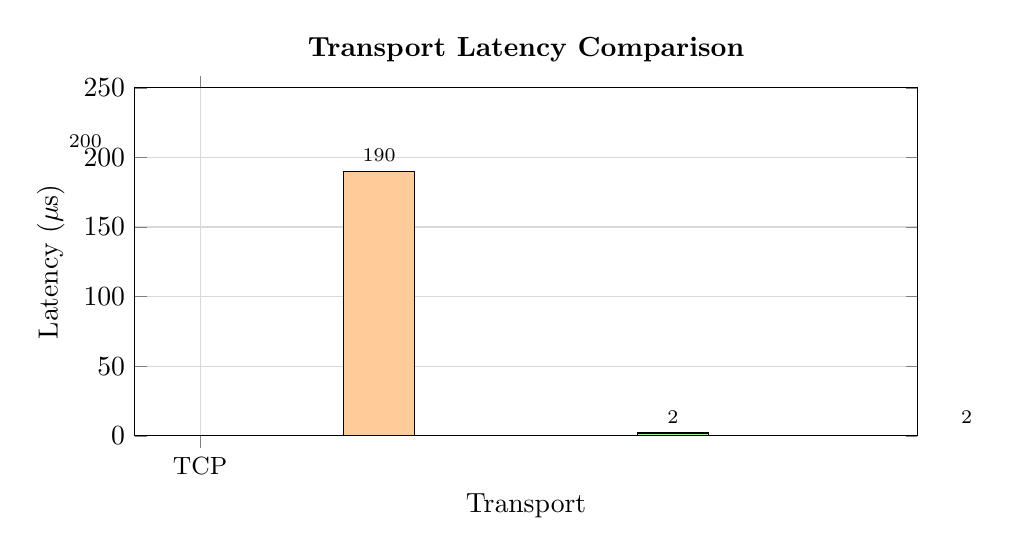
\begin{tikzpicture}
\begin{axis}[
    ybar,
    bar width=0.9cm,
    width=0.95\textwidth,
    height=6cm,
    ylabel={Latency ($\mu$s)},
    xlabel={Transport},
    ymin=0,
    ymax=250,
    ytick={0,50,100,150,200,250},
    symbolic x coords={TCP, Soft-RoCE, Hardware RoCE, TTPoe},
    xtick=data,
    x tick label style={font=\small},
    nodes near coords,
    nodes near coords align={vertical},
    every node near coord/.append style={font=\scriptsize},
    grid=major,
    grid style={gray!30},
    title={\textbf{Transport Latency Comparison}},
]
\addplot[fill=gray!40] coordinates {(TCP, 200)};
\addplot[fill=orange!40] coordinates {(Soft-RoCE, 190)};
\addplot[fill=green!40] coordinates {(Hardware RoCE, 2)};
\addplot[fill=purple!40] coordinates {(TTPoe, 2)};
\end{axis}
\end{tikzpicture}
\caption{Transport latency comparison---TCP baseline vs RDMA alternatives. Hardware RoCE and TTPoe achieve 100$\times$ lower latency than software solutions.}
\end{figure}

\section{EXO Distributed Inference Integration}

\subsection{Motivation}

In addition to the vLLM middleware, we integrated RDMA support into the exo distributed inference framework \cite{exo-github}, which provides an alternative approach to multi-node LLM serving using libp2p networking and peer-to-peer topology. While vLLM with Ray provides robust distributed inference, it requires complex session management between containers. The exo framework offers native peer-to-peer topology with automatic node discovery, an existing \texttt{RDMAConnection} type in its topology system (previously unimplemented), support for heterogeneous GPU clusters (e.g., mixing RTX 3090 and RTX 5090 nodes), and active development with a PyTorch backend (PR \#1284).

\subsection{Integration Architecture}

\begin{figure}[H]
\centering
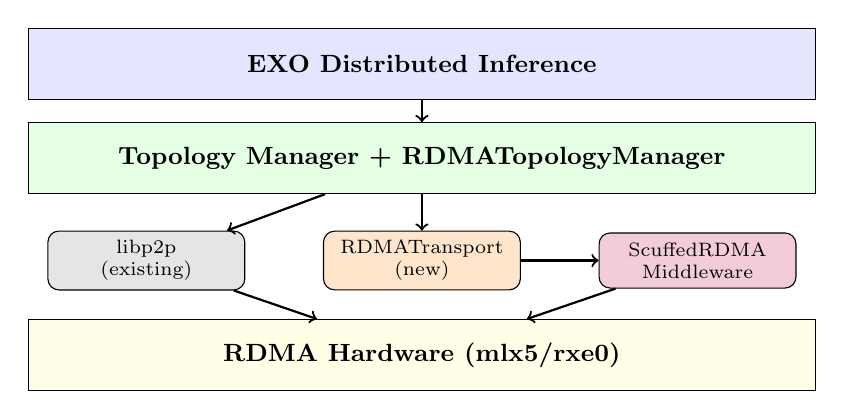
\begin{tikzpicture}[
    node distance=0.6cm,
    box/.style={rectangle, draw, rounded corners, minimum width=2.5cm, minimum height=0.7cm, align=center, font=\scriptsize},
    layer/.style={rectangle, draw, minimum width=10cm, minimum height=0.9cm, align=center, font=\small},
    arrow/.style={->, thick}
]
    % Top layer
    \node[layer, fill=blue!10] (exo) at (0,2.5) {\textbf{EXO Distributed Inference}};

    % Topology layer
    \node[layer, fill=green!10] (topo) at (0,1.3) {\textbf{Topology Manager + RDMATopologyManager}};

    % Transport boxes
    \node[box, fill=gray!20] (libp2p) at (-3.5,0) {libp2p\\(existing)};
    \node[box, fill=orange!20] (rdma) at (0,0) {RDMATransport\\(new)};
    \node[box, fill=purple!20] (middleware) at (3.5,0) {ScuffedRDMA\\Middleware};

    % Bottom layer
    \node[layer, fill=yellow!10] (hw) at (0,-1.2) {\textbf{RDMA Hardware (mlx5/rxe0)}};

    % Arrows
    \draw[arrow] (exo) -- (topo);
    \draw[arrow] (topo) -- (libp2p);
    \draw[arrow] (topo) -- (rdma);
    \draw[arrow] (rdma) -- (middleware);
    \draw[arrow] (libp2p) -- (hw);
    \draw[arrow] (middleware) -- (hw);
\end{tikzpicture}
\caption{EXO + RDMA integration architecture---RDMATransport wraps ScuffedRDMA middleware and integrates with exo's topology system}
\end{figure}

\subsection{Components Created}

Three new modules were created under the exo networking package:

\begin{table}[H]
\centering
\small
\begin{tabular}{@{}llp{6.5cm}@{}}
\toprule
\textbf{Module} & \textbf{Lines} & \textbf{Purpose} \\
\midrule
\texttt{rdma\_transport.py} & 369 & RDMA transport wrapper with discovery, connection management, and NCCL config \\
\texttt{rdma\_discovery\_integration.py} & 247 & Topology integration for automatic RDMA connection discovery \\
\texttt{\_\_init\_\_.py} & 27 & Module exports for networking package \\
\bottomrule
\end{tabular}
\caption{EXO RDMA integration components}
\end{table}

\subsection{Key Classes}

\subsubsection{RDMADiscovery}

The \texttt{RDMADiscovery} class discovers RDMA-capable interfaces on the local machine by invoking \texttt{rdma link show} and \texttt{ibv\_devinfo} as subprocesses and parsing their output. Its \texttt{get\_best\_interface()} method applies a priority ranking: hardware Mellanox devices (names matching \texttt{mlx5\_*}) are preferred over software Soft-RoCE devices (names matching \texttt{rxe*}), which in turn are preferred over any other RDMA-capable interface. This ensures that the highest-performance available transport is selected by default.

\subsubsection{RDMATransport}

The \texttt{RDMATransport} class wraps the ScuffedRDMA middleware for tensor transfer within the exo framework. Its \texttt{connect(peer\_node\_id, peer\_host, peer\_port)} method instantiates a \texttt{TransportSelector} in RoCE mode, retrieves the underlying transport object bound to the best local RDMA interface, and establishes a connection to the remote peer. The \texttt{get\_nccl\_config()} method returns the appropriate NCCL environment dictionary---falling back to TCP settings when no RDMA hardware is detected.

\subsubsection{RDMATopologyManager}

The \texttt{RDMATopologyManager} integrates with exo's topology system. Initialized with a node ID and the current topology graph, it uses \texttt{RDMADiscovery} to identify the best local RDMA interface. Its \texttt{discover\_and\_update()} method probes all known peers for RDMA connectivity and inserts \texttt{RDMAConnection} edges into the topology graph. The \texttt{get\_rdma\_peers()} method returns the list of peer node IDs reachable via RDMA by filtering outgoing edges for \texttt{RDMAConnection} instances.

\subsection{Leveraging Existing exo Types}

The integration leverages exo's existing \texttt{RDMAConnection} type, defined in the topology types module as a frozen model with source and sink RDMA interface fields. Although this type was present in exo's codebase, it had no concrete implementation until our integration. The placement utilities in exo's master module already check for \texttt{RDMAConnection} edges when selecting the jaccl communication backend, meaning our topology updates automatically influence backend selection for all-to-all collective operations.

\subsection{Integration Test Results}

Testing was performed on the Hydra control node, which lacks RDMA hardware, to validate the software path and graceful degradation. The middleware import, RDMA transport import, RDMA discovery (correctly reporting unavailable), TCP transport availability, NCCL configuration generation, and RDMA connection manager all passed successfully. The topology integration test failed due to a Python 3.10 incompatibility with the \texttt{Self} type hint (available in 3.11+); this can be resolved by importing \texttt{Self} from \texttt{typing\_extensions} or updating the type annotations.

\subsection{Cluster Deployment}

\begin{table}[H]
\centering
\small
\begin{tabular}{@{}llll@{}}
\toprule
\textbf{Node} & \textbf{IP} & \textbf{GPUs} & \textbf{RDMA Status} \\
\midrule
Chimera & 192.168.1.150 & 3$\times$ RTX 3090 & Soft-RoCE (rxe0) \\
Cerberus & 192.168.1.233 & 2$\times$ RTX 5090 & Soft-RoCE (rxe0) \\
Hydra & 192.168.1.100 & None (control) & N/A \\
\bottomrule
\end{tabular}
\caption{Cluster configuration for exo + RDMA testing}
\end{table}

\subsection{Source References}

\begin{itemize}[noitemsep]
    \item \textbf{exo repository}: \url{https://github.com/exo-explore/exo}
    \item \textbf{PyTorch backend PR}: \url{https://github.com/exo-explore/exo/pull/1284}
\end{itemize}

\section{Limitations and Future Work}

\subsection{Current Limitations}

\begin{itemize}[noitemsep]
    \item \textbf{TTPoe integration}: The character device interface requires a custom NCCL plugin for full integration with collective operations
    \item \textbf{pyverbs dependency}: The RoCE transport requires rdma-core compiled with Python bindings, which is not available in all distributions
    \item \textbf{Module permissions}: TTPoe module loading requires root access, complicating containerized deployments
\end{itemize}

\subsection{Planned Enhancements}

\begin{itemize}[noitemsep]
    \item Implement an NCCL socket plugin for TTPoe transport
    \item Add hardware RoCE detection and automatic configuration
    \item Create a Prometheus metrics exporter for transport monitoring
    \item Integrate with vLLM tensor transfer hooks for fine-grained control
    \item Test the middleware with Mellanox ConnectX NICs for hardware RoCE benchmarks
    \item Load TTPoe modules on the cluster and measure actual end-to-end latency
    \item Instrument vLLM tensor transfers for telemetry collection
    \item Implement adaptive hot/cold tensor classification with weighted flow allocation
    \item Run Llama 4 Scout benchmarks across all transports in production configuration
\end{itemize}

\section{Summary}

This work delivers a complete transport middleware layer for distributed LLM inference, together with integration into the exo peer-to-peer framework:

\begin{itemize}[noitemsep]
    \item \textbf{Transport abstraction}: A unified API across TCP, RoCE, and TTPoe backends
    \item \textbf{Dynamic selection}: Runtime transport switching via environment variables or CLI flags
    \item \textbf{NCCL integration}: Automatic environment configuration for vLLM/Ray clusters
    \item \textbf{Benchmark tooling}: A unified suite for systematic transport comparison
    \item \textbf{Cluster management}: Scripts for multi-node deployment with transport flags
    \item \textbf{EXO integration}: RDMA transport modules for exo distributed inference (639 lines of new code)
    \item \textbf{Topology discovery}: Automatic RDMA connection discovery and topology graph updates
\end{itemize}

The middleware establishes the foundation for adaptive transport selection in distributed LLM inference. The exo integration provides an alternative to vLLM+Ray with native peer-to-peer RDMA support, enabling testing on heterogeneous GPU clusters (RTX 3090 + RTX 5090).

\begin{thebibliography}{99}

\bibitem{exo-github}
exo-explore. (2025). \textit{exo: Run your own AI cluster at home with everyday devices}. \url{https://github.com/exo-explore/exo}

\bibitem{rdma-core}
Linux RDMA. (2024). \textit{rdma-core Documentation}. \url{https://github.com/linux-rdma/rdma-core}

\bibitem{ttpoe-repo}
Tesla, Inc. (2024). \textit{TTPoe: Time-Triggered Protocol over Ethernet}. \url{https://github.com/teslamotors/ttpoe}

\bibitem{nccl-docs}
NVIDIA. (2024). \textit{NCCL Documentation}. \url{https://docs.nvidia.com/deeplearning/nccl/user-guide/docs/}

\bibitem{vllm-docs}
vLLM Team. (2024). \textit{vLLM Documentation}. \url{https://docs.vllm.ai/}

\bibitem{ray-docs}
Anyscale. (2024). \textit{Ray Documentation}. \url{https://docs.ray.io/}

\bibitem{pyverbs-docs}
Linux RDMA. (2024). \textit{pyverbs - Python bindings for rdma-core}. \url{https://github.com/linux-rdma/rdma-core/tree/master/pyverbs}

\end{thebibliography}

\end{document}
